\documentclass[english]{article}
\usepackage{a4,babel}
\usepackage[utf8]{inputenc}
\usepackage[T1]{fontenc}
\usepackage{graphicx,amssymb,amstext,amsmath,listings,color}
\usepackage{setspace,varioref,url,placeins}

\def\author			{Ludvig Widman(dit06lwn), Emil Eriksson(c07een)}
\def\email			{}
\def\course			{Distributed Systems. 5DV020, HT09}
\def\delivery		{Assignment part 1}
\def\trivialname	{Analysis and design}
\def\tutor			{Lars Larsson, Daniel Henriksson}
\def\myabstract	{}

%-----------------------------------------------------------
\begin{document}
%-----------------------------------------------------------
\begin{titlepage}
\noindent
\course \\
\author \\

\noindent
Tutors: \tutor \\
Date: \today \\


\begin{center}
		\vspace{20mm}
        \Huge \delivery \\
        \vspace{5mm}
        \Huge \trivialname \\
        \vspace{70mm}
        
\end{center}
\end{titlepage}
%-----------------------------------------------------------
\thispagestyle{empty}
\pagenumbering{roman}
\tableofcontents
\newpage
\pagenumbering{arabic}

\setstretch{1.3}	% Radavstånd
% Mellanrum mellan stycken, inget indrag
\setlength{\parindent}{0pt}
\setlength{\parskip}{1ex plus 0.5ex minus 0.2ex}


%-----------------------------------------------------------
\section{Bonus Level}
We intend to solve bonus level two with dynamic groups. 


%-----------------------------------------------------------
\section{Tools and language for implementation}
Since the clear recommendation is to use Java and Java RMI we have decided to follow the recommendation. While there are languages that would be more interesting and easier to design GUIs in (cocoa/objective c), Java is more easily ported and the available help from lecturers also helped tip the balance in Java's favor.

JUnit will be used for unit testing and logging will be done through the log4j-package. 

%-----------------------------------------------------------
\section{Project plan}
\begin{tabular}{|l|l|l|}
\hline
Date	&	Milestone	&	Content \\
\hline
11 Sept	&	Part 1 due	&	Written project plan \\
18 Sept &	Milestone 1 &	Create all interfaces \\ 
						&&	Build dataobjects \\
						&&	Design GUI mockups for test app \\
25 Sept &	Milestone 2 & 	Implement basic methods like non-ordered ordering and non-reliable multicast. \\
2 Oct	&	Milestone 3 & 	Implement advanced methods like total ordering and reliable multicast. \\
9 Oct	&	Milestone 4 & 	Implement GUI-application and debug mode. \\
16 Oct	&	Milestone 5 & 	Resolve distributed problems. \\ && Write on the report.\\ && Make test protocol. \\
23 Oct	&	Finalization 	& Everything should be finished. Minor adjustments. \\
27 Oct	&	Hand in report 	& \\
28-30 Oct & Demonstration	& \\
\hline
\end{tabular}

%-----------------------------------------------------------
\section{Design}


% TODO: We should design/workout how we will do debugging

\subsection{GCom}
A framework (middleware) for communicating between distributed nodes within groups.
This module exposes the functionality of the other modules that are part of GCom so that referencing them directly should not be needed in order to use them.
%	(Interface from previous year http://www.cs.umu.se/kurser/5DV020/HT08/GCom.java)

\subsubsection{Interface}
\begin{itemize}
\item[+]  joinGroup(String groupName) \\
	Contact RMI registry and get group-leader \\
	Contact group-leader

\item[+]  createGroup(String groupName)
	Register at RMI registry

\item[+]  removeGroup(String groupName) \\
	Removes the group from the RMI registry

\item[+] leave(String groupName) \\
	Send GroupView excluding sending Member

\item[+]  listGroups \\
	Ask registry

\item[+]  listMembers(String groupName)

\item[+]  sendMessage(String groupName, Message) \\
	Sends a message to the specified group via CommunicationModule

\item[+]  connectToRegistry(String host, int port) \\
	Connects to a RMI registry
\end{itemize}

\subsection{CommunicationModule}
Sends and receives messages to and from other processes. This module must support both reliable and basic multicast. Received data is sent to the MessageOrderingModule. The GroupManagementModule is also notified with the senders process ID. 

\subsubsection{Interface}
\begin{itemize}
\item[+] receive(Message)
	This method is called remotely by other nodes when sending messages to this node.

\item[+] send(Group, Message) \\
	Look up communication type in group \\
	Look up group members

\item[-] multicastB
	Private method used internally to perform a basic multicast.

\item[-] multicastR
	Private method which uses multicastB to perform a reliable multicast.

\end{itemize}

\subsection{MessageOrderingModule}
Sorts incoming messages and makes sure that they're delivered according to the specified order (Non-ordered, FIFO, Causal, Total, Causal-Total). Non-ordered is the main class and the other ordering methods is implemented as subclasses. 

\subsubsection{Interface}
\begin{itemize}
\item[+] queueMessage(Message)
\end{itemize}

\subsection{GroupManagementModule}
The GroupManagementModule contains collection of Group objects. It monitors if a process stops responding. Notifies changes in the states to all members of the group (via the CommunicationModule). The GroupManagementModule also resolves group names to a list of members.

\subsubsection{Interface}
\begin{itemize}
\item[+] addGroup(String groupName)
\item[+] removeGroup(String groupName)
\item[+] listGroups
\end{itemize}

\subsection{Group}
Stores a group's state and group members.

\subsubsection{Interface}
\begin{itemize}
\item[+] addMember \\
	Adds the member to the member list
\item[+]  removeMember \\
	Removes the member from the member list
\item[+]  listMembers
\item[+]  update(ProcessID) \\
	Updates the last seen vector time for the process
\end{itemize}


\subsection{GUI}
The GUI class contains the application that uses GCom and is mostly used for testing and demonstration. We intend to write some kind of simple chat application. The GUI registers listeners in the GCom class to get information. 


\subsection{Message}
The Message is a basic data object which can be serialized. It contains a Vector clock, a destination group, message type and the actual message. 

\subsection{RMI Registry}
A central RMI-registry. Single point of failure. Leader registers and unregisters group. 

\begin{figure}[h]
	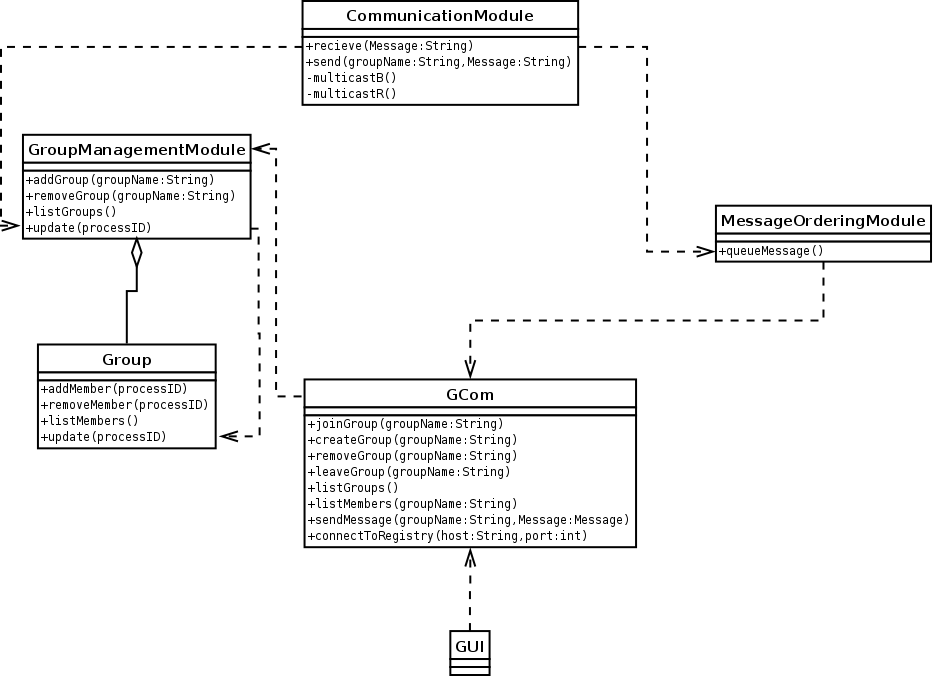
\includegraphics[width=150mm]{klasser.png}
	\caption{How the modules are related.}
\end{figure}

%-----------------------------------------------------------
\section{Use cases}

A few of the scenarios that might arise during using and testing GCom.

\subsection{A node creates a new group}
When a node wants to create a new group, it connects to the RMI-Registry and leaves a reference to itself under the name of the channel.

If this succeeds it sets itself as the group leader and adds itself to it's view of the group in the GroupManagementModule.

If the registration fails an exception indicating if the name was already taken or the RMI-Registry was unresponsive is thrown.

\subsection{A group leader removes a group}
The leader removes all members from it's view of the group in GroupManagementModule and then sends this updated view to all members of the group via the CommunicationModule. It then unregisters the group name in the registry.

\subsection{A member joins a group}
When joining a group the prospective member connects to the RMI-Registry and gets a reference to the group leader and sends it a join request. The leader adds the new member to it's view of the group and then sends this updated view to all members of the group, including the new member. When the new member receives the updated view it knows it is part of the group.

\subsection{A member leaves group}
When a member wants to leave a group it sends a group view excluding itself to all the members (including the group-leader) of the group.

\subsection{Send message to a group}
First a list of all members in the group is obtained from the GroupManagementModule and then the message is sent to all of the members.

%\subsection{Member receives message with much later time-stamp than previous message}
%TODO: Design a way for a node to request an older message

\subsection{Group-leader leaves group}
When the group-leader leaves the group the remaining members starts electing a new group leader by creating a semi-random (and unique) value and sending this to all other nodes in an election-message.

%TODO: A crashed node could make a group-leader election fail.
When a node receives election-messages it compares the value in the incoming message with the value it created and sends the larger of these to all other nodes. When a node has received messages with it's own value from all members of the group it sets itself as group-leader and registers with the RMI-Registry.

For now we do not take into account that a node might crash during the election.

If the group-leader leaves a single member behind this node realizes it is alone in the group and sets itself as group-leader and registers with the registry.

\subsection{The last member in a group leaves}
When the last member of a group leaves it is the group-leader and it unregisters itself from the registry.

%-----------------------------------------------------------
\section{Fault tolerance}

\subsection{Detecting crashed members}
The GroupManagementModule gets notified when a message is received and can therefore keep track of the time since the last message from a process, measured in vector time. If a process does not send anything for a long time it will be marked as crashed and removed from the group list.

\subsection{If the registry restarts or is unresponsive}
The leader of each group occasionally checks that the group is registered in the RMI-registry. If the registry has restarted for some reason the leader will re-register the group.

\subsection{If the group leader crashes}
If the group leader crashes the group will detect that no messages arrive from the leader and then elect a new leader. 

\subsection{If the last member of a group crashes}
If the last member of a group crashes no one will unregister the group.
This will potentially lead to a lot of "dead" references in the registry if there is a bug causing nodes to crash when they are the last to leave a group. In order to counter this some extra testing will be done to make sure that nodes behave when leaving and unregistering with the registry.
If the time allows we will try to implement a way to clear out old references in the registry (other than restarting it periodically).

\subsection{Netsplit}
If the group is split in two partitions, due to a cable failure or similar, the partition with the leader will continue to work as before. The other partition will elect a new leader when they discover that they no longer receive messages from the leader.
The new leader will try to reregister the group in the registry. The leader for the other part will do the same and therefore compete over the reference in the registry. Because of this newcomers will join the group having the reference in the registry at the time the node connects.

%-----------------------------------------------------------
\section{Requirement Specification}

\subsection{Group management}
\begin{description}
\item[REQUIRED] External processes must be able to find and connect to group leaders via a RMI registry.

\item[REQUIRED] The group leader must regularly make sure that the group and leader is registered in the RMI registry.

\item[REQUIRED] Any process must be able to create a new group and register itself as leader in the registry.

\item[REQUIRED] Any process must be able to join a group by connecting to the group leader.

\item[REQUIRED] Every process in a group must notify the other processes of any known changes to the group composition.

\item[REQUIRED] Every process must keep track of the members of all the groups it's a member of.

\item[REQUIRED] Every process must monitor if another process in the group stops responding and report a corresponding change in group composition.

\item[REQUIRED] If the leader of the group leaves or crashes a new leader must be elected in the group.
\end{description}


\subsection{Communication}
\begin{description}
\item[REQUIRED] It must be possible to send messages to the members of joined group.

\item[REQUIRED] Both non-reliable and reliable multicast must be supported for sending messages.

\item[REQUIRED] The communication method chosen by the group creator (reliable or non-reliable multicast) must be used when communicating in a group.

\item[REQUIRED] Every message must contain a updated vector clock.
\end{description}


\subsection{Message Ordering}
\begin{description}
\item[REQUIRED] Any message must arrive in proper order (according to the selected sorting requirements).

\item[REQUIRED] A message must not be delivered until all previous messages are delivered if the message ordering demands so.
\end{description}



%-----------------------------------------------------------
\section{Limitations}
\begin{itemize}
\item The RMI-registry is a single point of failure. If the registry crashes no processes can find or join groups. 

\item If a group is split in two parts due to network failure and both parts still have contact  with the registry bad things will happen. This is assumed to never happen.

\item All processes are assumed to be good. If a process starts to lie or send malicious messages bad things will happen.
\end{itemize}

\end{document}
